\section{Space of translations}

\frame{
	\frametitle{Model of translational equivalences}
	
	Describes the process of generating translations of a given input
	\begin{itemize}
		\item constrains and characterises \\
		the set of possible translation derivations
	\end{itemize}
	
	\pause
	
	\begin{block}{Phrase-based MT}
	we observe an input, segment it into phrases, permute the phrases into  target language word-order, and finally, translate segments independently
	\end{block}
	
	\pause

	\begin{block}{Hierarchical MT}
	we parse the input with a CFG, then translate (using synchronous rules) each and every edge independently
	\end{block}
	
}

\frame{
	\frametitle{CFGs and FSAs}
	
	Compactly represent the set of translations
	\begin{itemize}
		\item keep the representation cost a tractable (polynomial) function of the input length
	\end{itemize}
	
	~
	
	
	Phrase-based MT $O(n^2 2^d)$
	
	~
	
	Hierarchical MT $O(n^3)$
}

\frame{
	\frametitle{Independence assumptions}
	
	Translation rules (flat or CFG) are applied independently
	
	\only<2>{
	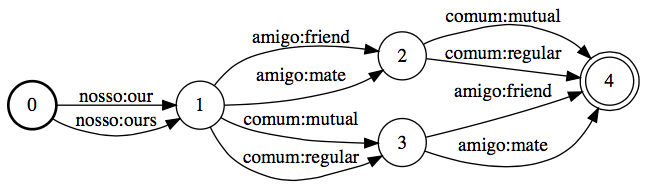
\includegraphics[scale=0.4]{img/fsa}
	}
	\only<3>{
	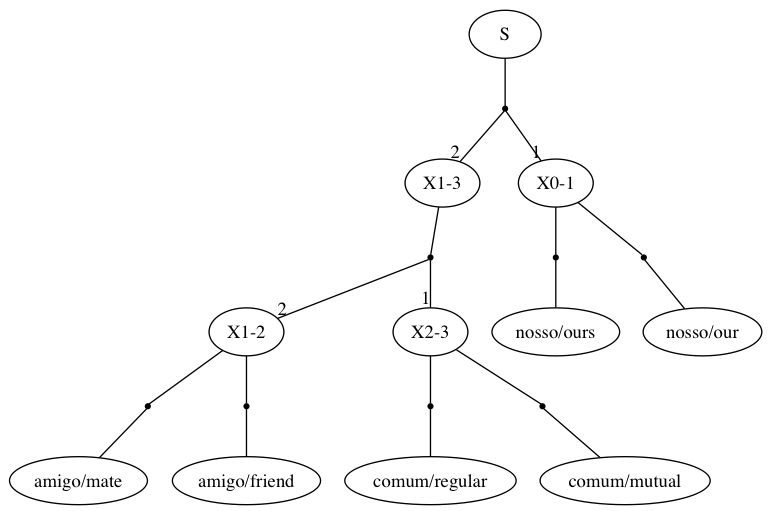
\includegraphics[scale=0.4]{img/cfg}
	}
	
}

